% --- SLIDE 11: Connecting Degenerate Strings to DAGs ---
\begin{frame}{From Degenerate Strings to Weighted DAGs}
    \framesubtitle{A New Perspective}

    Recall our degenerate string $X$:
    \begin{figure}[h!]
        \centering
        % Usa la figura della stringa degenere che hai già definito
        \begin{tabular}{c@{\hskip 0.5em}c@{\hskip 0.5em}c@{\hskip 0.5em}c@{\hskip 0.5em}c}
            $X = $                                                                           & $\Bigg\{\,\begin{matrix}\texttt{A}\\\texttt{C}\\\texttt{G}\end{matrix}\,\Bigg\}$ &
            $\Bigg\{\,\begin{matrix}\texttt{A}\\\texttt{T}\end{matrix}\,\Bigg\}$             &
            $\Bigg\{\,\begin{matrix}\texttt{T}\\\texttt{C}\\\texttt{A}\end{matrix}\,\Bigg\}$ &
            $\Bigg\{\,\begin{matrix}\texttt{A}\\\texttt{G}\end{matrix}\,\Bigg\}$                                                                                                                        \\
                                                                                             & $X_1$                                                                            & $X_2$ & $X_3$ & $X_4$
        \end{tabular}
    \end{figure}

    \uncover<2->{
        \begin{block}{Key Idea}
            We can model queries on $X$ by constructing a specific node-weighted Directed Acyclic Graph (DAG) $G_c$ for a target character $c$.
        \end{block}
    }

    \uncover<3->{
        \begin{itemize}
            \item<3-> \textbf{Vertices $V_c$}: Source $s$ + one node $v_{k,a}$ for each character $a \in X_k$ at each position $k$.
            \item<4-> \textbf{Weights $w_c$}: $w_c(s)=0$. $w_c(v_{k,a}) = 1$ if $a = c$, else $0$. (Highlights occurrences of $c$).
            \item<5-> \textbf{Edges $E_c$}: Connect $s$ to $k=1$. Connect all $v_{k,a}$ to all $v_{k+1,b}$. (Represents sequence adjacency).
        \end{itemize}
    }

\end{frame}

% % --- SLIDE 12: Visualizing the DAG Construction (Example: c = A) --- USING \pause
% \begin{frame}{Visualizing the DAG Construction (Example: c = A)}
%     \framesubtitle{Building $G_A$ Step-by-Step}

%     \begin{figure}[h!]
%         \centering
%         \resizebox{\textwidth}{!}{% Resize to fit slide width if needed
%             \begin{tikzpicture}[
%                     node distance=2.8cm and 1.0cm, % x distance and y distance
%                     % Define node styles explicitly for clarity
%                     node_style/.style={circle, draw, thick, minimum size=7mm, inner sep=0pt},
%                     weight_one/.style={node_style, fill=yellow!50},
%                     weight_zero/.style={node_style, fill=gray!20},
%                     source_node/.style={node_style, fill=red!60},
%                     % Edge style
%                     edge_style/.style={->, >=latex, thin, gray}
%                 ]

%                 % --- Step 1: Draw Source Node ---
%                 \node[source_node] (s) at (0, 0) {$s$};

%                 % --- Step 2: Draw Level 1 Nodes and Edges from s ---
%                 \node[weight_one] (v1A) at (2, 2) {\tiny (1,A)}; \node[below=1pt of v1A] {\tiny w=1};
%                 \node[weight_zero](v1C) at (2, 0) {\tiny (1,C)}; \node[below=1pt of v1C] {\tiny w=0};
%                 \node[weight_zero](v1G) at (2,-2) {\tiny (1,G)}; \node[below=1pt of v1G] {\tiny w=0};
%                 \foreach \v in {v1A, v1C, v1G} { \draw[edge_style] (s) -- (\v); }

%                 \pause % Wait for click

%                 % --- Step 3: Draw Level 2 Nodes and Edges from Level 1 ---
%                 \node[weight_one] (v2A) at (4.8, 1) {\tiny (2,A)}; \node[below=1pt of v2A] {\tiny w=1};
%                 \node[weight_zero](v2T) at (4.8,-1) {\tiny (2,T)}; \node[below=1pt of v2T] {\tiny w=0};
%                 \foreach \u in {v1A, v1C, v1G} {
%                         \foreach \v in {v2A, v2T} { \draw[edge_style] (\u) -- (\v); }
%                     }

%                 \pause % Wait for click

%                 % --- Step 4: Draw Level 3 Nodes and Edges from Level 2 ---
%                 \node[weight_zero] (v3T) at (7.6, 2) {\tiny (3,T)}; \node[below=1pt of v3T] {\tiny w=0};
%                 \node[weight_zero](v3C) at (7.6, 0) {\tiny (3,C)}; \node[below=1pt of v3C] {\tiny w=0};
%                 \node[weight_one](v3A) at (7.6,-2) {\tiny (3,A)}; \node[below=1pt of v3A] {\tiny w=1};
%                 \foreach \u in {v2A, v2T} {
%                         \foreach \v in {v3T, v3C, v3A} { \draw[edge_style] (\u) -- (\v); }
%                     }

%                 \pause % Wait for click

%                 % --- Step 5: Draw Level 4 Nodes and Edges from Level 3 ---
%                 \node[weight_one] (v4A) at (10.4, 1) {\tiny (4,A)}; \node[below=1pt of v4A] {\tiny w=1};
%                 \node[weight_zero](v4G) at (10.4,-1) {\tiny (4,G)}; \node[below=1pt of v4G] {\tiny w=0};
%                 \foreach \u in {v3T, v3C, v3A} {
%                         \foreach \v in {v4A, v4G} { \draw[edge_style] (\u) -- (\v); }
%                     }

%             \end{tikzpicture}
%         } % End resizebox
%     \end{figure}

%     % Il testo finale appare dopo l'ultimo pause implicito
%     \begin{center}
%         This connection motivates the core topic: \\ \textbf{Efficient data structures for path-based queries on general node-weighted DAGs.}
%     \end{center}

% \end{frame}


% \begin{frame}{Mathematical Framework: Weighted DAGs}
%     \framesubtitle{Basic Definitions}
%     Given a path $P=(v_0=s, \dots, v_k=v)$ we define $W(P) = \sum_{j=1}^{k} w(v_j)$ as the cumulative weight of the path $P$.
%     % \begin{block}{Path and Path Weight}
%     %     \begin{itemize}
%     %         \item Path $P = (v_0=s, \dots, v_k=v)$.
%     %         \item Weight $W(P) = \sum_{j=1}^{k} w(v_j)$.
%     %     \end{itemize}
%     % \end{block}
%     \begin{figure}[h!]
%         \centering
%         \resizebox{0.95\textwidth}{!}{% Scale to fit column
%             \begin{tikzpicture}[
%                 node distance=1.5cm and 1cm,
%                 base_node/.style={circle, draw=black, thick, minimum size=8mm, inner sep=0pt, font=\sffamily},
%                 root_node/.style={base_node, fill=red!60, text=black},
%                 edge_style/.style={->, >={Stealth[length=2mm]}, thick, draw=black}
%                 ]
%                 % Nodes showing only their weight w(v)
%                 \node[root_node] (0) at (0, 2) {0};
%                 \node[base_node] (1) at (1.5, 0) {1};
%                 \node[base_node] (3) at (1.5, 4) {3};
%                 \node[base_node] (6) at (3.5, 1.5) {6};
%                 \node[base_node] (7) at (4.5, 0) {7};
%                 \node[base_node] (2) at (5.5, 4) {2};
%                 \node[base_node] (9) at (6.5, 2) {9};
%                 \node[base_node] (5) at (9, 0.5) {5};
%                 \node[base_node] (10) at (8.5, 5) {10};
%                 \node[base_node] (8) at (11, 3) {8};

%                 % Edges (same as before)
%                 \draw [edge_style] (0) -- (1); \draw [edge_style] (0) -- (3);
%                 \draw [edge_style] (1) -- (6); \draw [edge_style] (1) -- (7);
%                 \draw [edge_style] (3) -- (2); \draw [edge_style] (3) -- (6);
%                 \draw [edge_style] (6) -- (2); \draw [edge_style] (6) -- (9);
%                 \draw [edge_style] (7) -- (5); \draw [edge_style] (7) -- (9);
%                 \draw [edge_style] (2) -- (10);
%                 \draw [edge_style] (9) -- (5); \draw [edge_style] (9) -- (8);
%                 \draw [edge_style] (10) -- (8); \draw [edge_style] (5) -- (8);
%             \end{tikzpicture}
%         } % End resizebox
%     \end{figure}

%     % \begin{columns}[T]
%     %     % Colonna sinistra: Definizioni
%     %     \begin{column}{0.5\textwidth}
%     %         \begin{block}{Weighted DAG $G=(V, E, w)$}
%     %             \begin{itemize}
%     %                 \item $V$: Finite set of vertices.
%     %                 \item $E$: Directed edges, no cycles.
%     %                 \item $w: V \to \mathbb{N}_0$: Non-negative node weights.
%     %                 \item Unique source $s$ with $w(s)=0$.
%     %             \end{itemize}
%     %         \end{block}
%     %         \begin{block}{Path and Path Weight}
%     %             \begin{itemize}
%     %                 \item Path $P = (v_0=s, \dots, v_k=v)$.
%     %                 \item Weight $W(P) = \sum_{j=1}^{k} w(v_j)$.
%     %             \end{itemize}
%     %         \end{block}
%     %     \end{column}

%     %     % Colonna destra: Figura Esempio DAG (solo pesi)
%     %     \begin{column}{0.5\textwidth}
%     %         \begin{figure}[h!]
%     %             \centering
%     %             \resizebox{0.95\textwidth}{!}{% Scale to fit column
%     %                 \begin{tikzpicture}[
%     %                     node distance=1.5cm and 1cm,
%     %                     base_node/.style={circle, draw=black, thick, minimum size=8mm, inner sep=0pt, font=\sffamily},
%     %                     root_node/.style={base_node, fill=red!60, text=black},
%     %                     edge_style/.style={->, >={Stealth[length=2mm]}, thick, draw=black}
%     %                     ]
%     %                     % Nodes showing only their weight w(v)
%     %                     \node[root_node] (0) at (0, 2) {0};
%     %                     \node[base_node] (1) at (1.5, 0) {1};
%     %                     \node[base_node] (3) at (1.5, 4) {3};
%     %                     \node[base_node] (6) at (3.5, 1.5) {6};
%     %                     \node[base_node] (7) at (4.5, 0) {7};
%     %                     \node[base_node] (2) at (5.5, 4) {2};
%     %                     \node[base_node] (9) at (6.5, 2) {9};
%     %                     \node[base_node] (5) at (9, 0.5) {5};
%     %                     \node[base_node] (10) at (8.5, 5) {10};
%     %                     \node[base_node] (8) at (11, 3) {8};

%     %                     % Edges (same as before)
%     %                     \draw [edge_style] (0) -- (1); \draw [edge_style] (0) -- (3);
%     %                     \draw [edge_style] (1) -- (6); \draw [edge_style] (1) -- (7);
%     %                     \draw [edge_style] (3) -- (2); \draw [edge_style] (3) -- (6);
%     %                     \draw [edge_style] (6) -- (2); \draw [edge_style] (6) -- (9);
%     %                     \draw [edge_style] (7) -- (5); \draw [edge_style] (7) -- (9);
%     %                     \draw [edge_style] (2) -- (10);
%     %                     \draw [edge_style] (9) -- (5); \draw [edge_style] (9) -- (8);
%     %                     \draw [edge_style] (10) -- (8); \draw [edge_style] (5) -- (8);
%     %                 \end{tikzpicture}
%     %             } % End resizebox
%     %         \end{figure}
%     %     \end{column}
%     % \end{columns}
% \end{frame}

% --- SLIDE 13: Path Weight Aggregation: The O-Set Definition ---
\begin{frame}{Path Weight Aggregation: The $\mathcal{O}$-Set}
    \framesubtitle{Capturing All Path Weights}
    Given a path $P=(v_0=s, \dots, v_k=v)$ we define $W(P) = \sum_{j=1}^{k} w(v_j)$
    \begin{alertblock}{Goal}
        Characterize the set of \alert{all possible distinct} cumulative path weights arriving at each node.
    \end{alertblock}
    % \vspace{1em}
    \pause
    \begin{block}{$\mathcal{O}$-Set Definition (Recursive)}
        \begin{itemize}
            \item \textbf{Base Case (Source):} $\mathcal{O}_s = \{0\}$
            \item \textbf{Recursive Step ($v \neq s$):}
                  \[ \mathcal{O}_v = \bigcup_{u \in Pred(v)} \{ y + w(v) \mid y \in \mathcal{O}_u \} = \{ W(P) \mid P \in Path(s, v) \}  \]
                  Keep only \alert{distinct} values. Store as a sorted sequence.
        \end{itemize}
    \end{block}
    % The set $\mathcal{O}_v$ contains \emph{exactly} the weights $W(P)$ for all paths $P$ from source $s$ to $v$.
    % \[ \mathcal{O}_v = \{ W(P) \mid P \in Path(s, v) \} \]

\end{frame}

% --- SLIDE 14: O-Set Construction Example ---
\begin{frame}{$\mathcal{O}$-Set Construction Example}
    \framesubtitle{Visualizing the Recursive Definition}
    \vspace{-0.5em}
    \begin{figure}[hbtp]
        % \centering
        % Replace TikZ with sequential images
        \only<1>{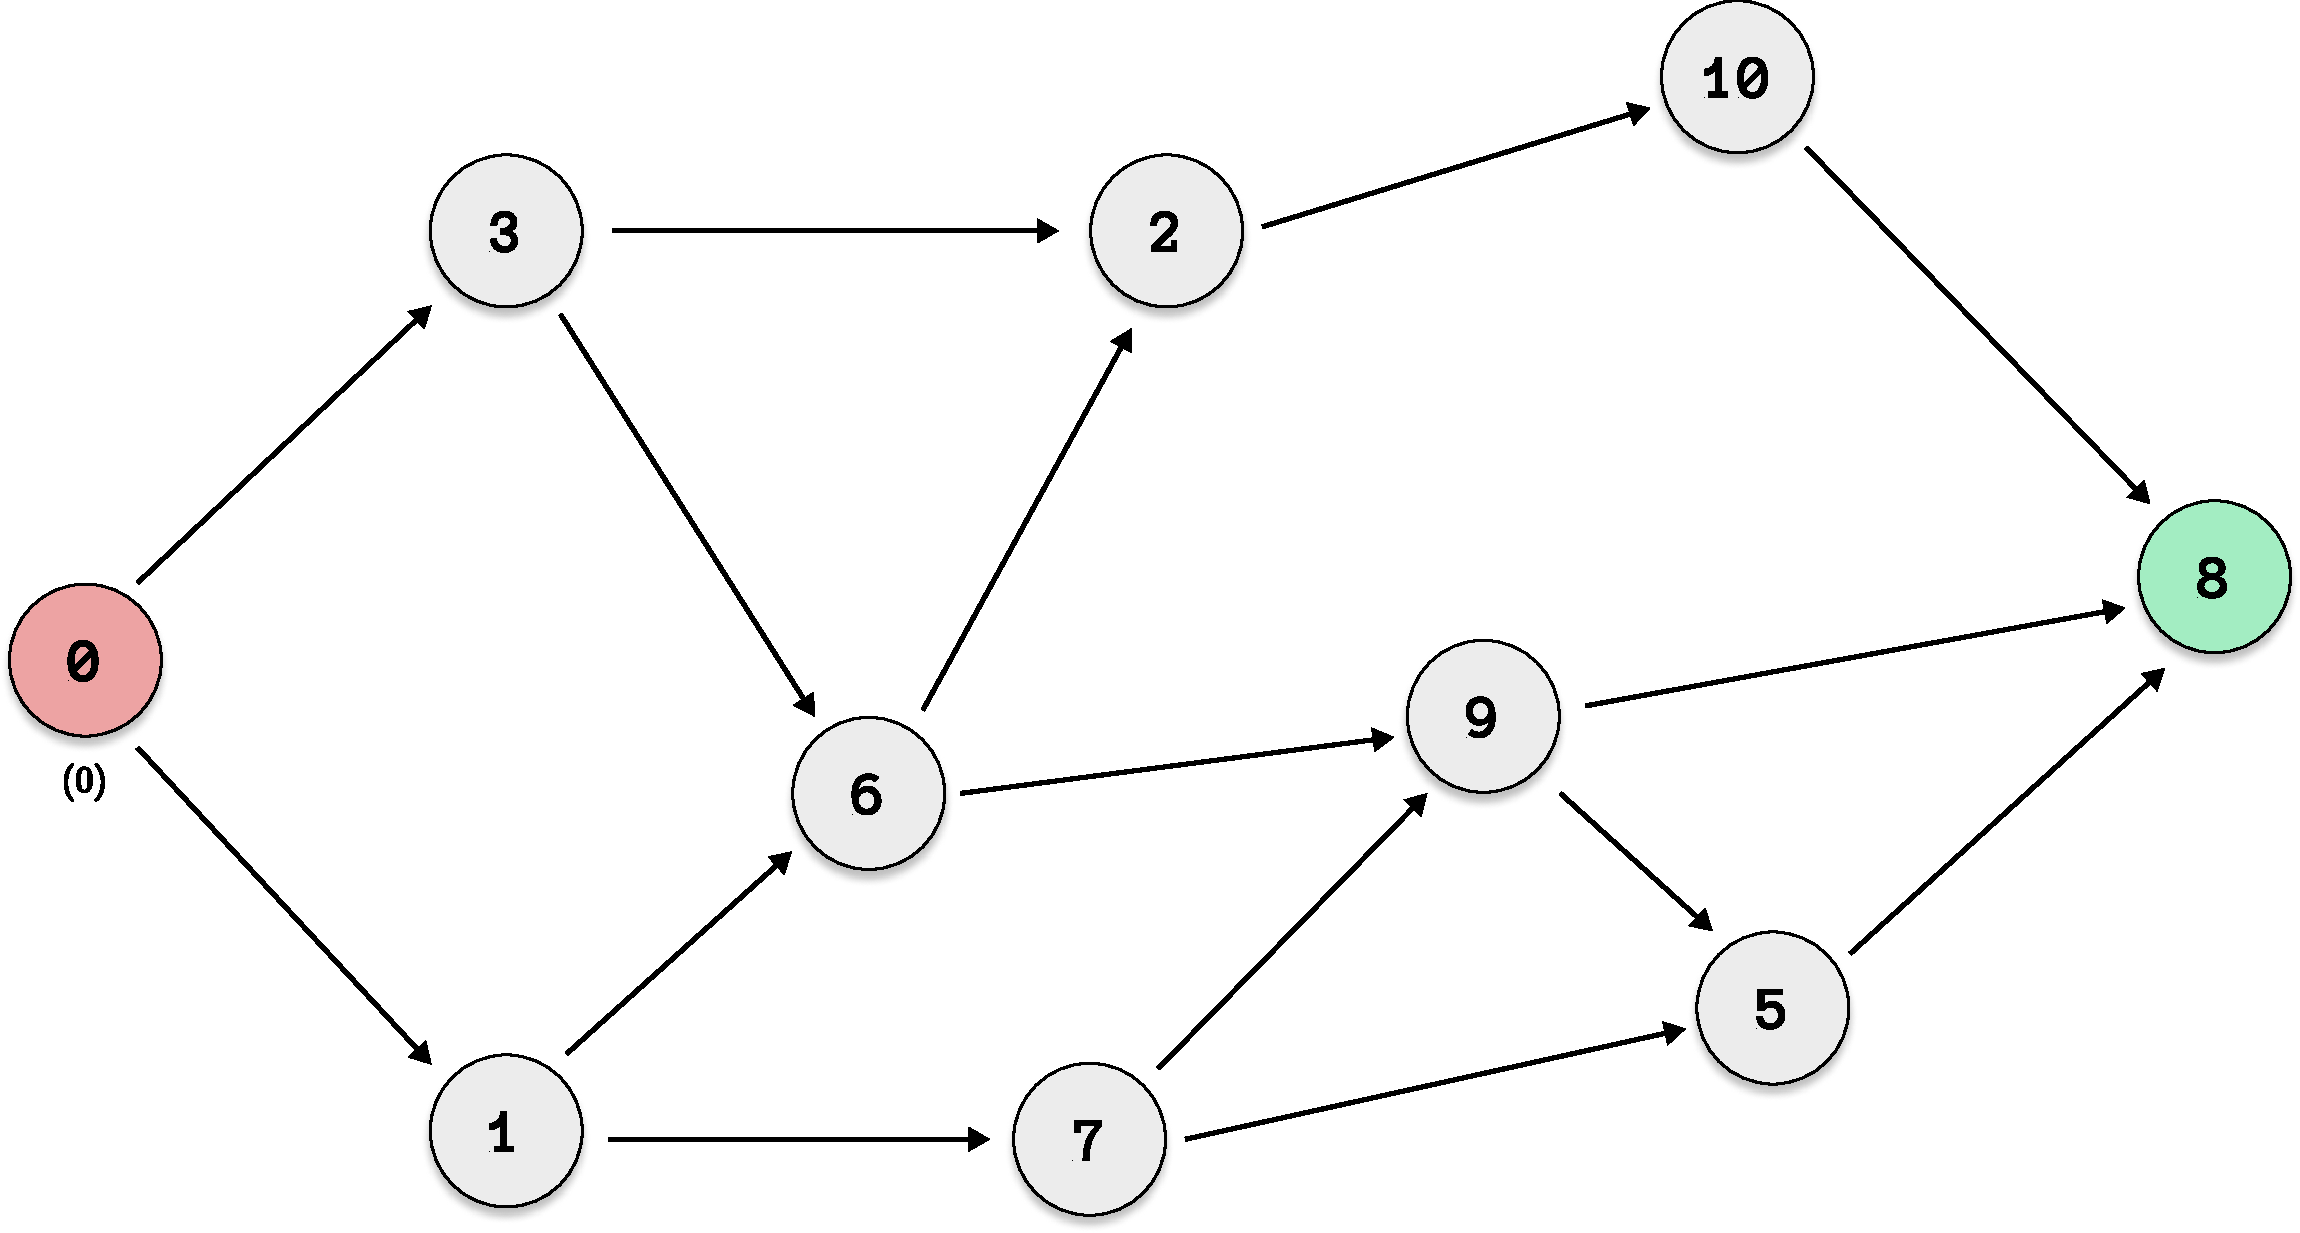
\includegraphics[width=0.85\textwidth]{assets/dag_explicit1.pdf}}
        % \only<2>{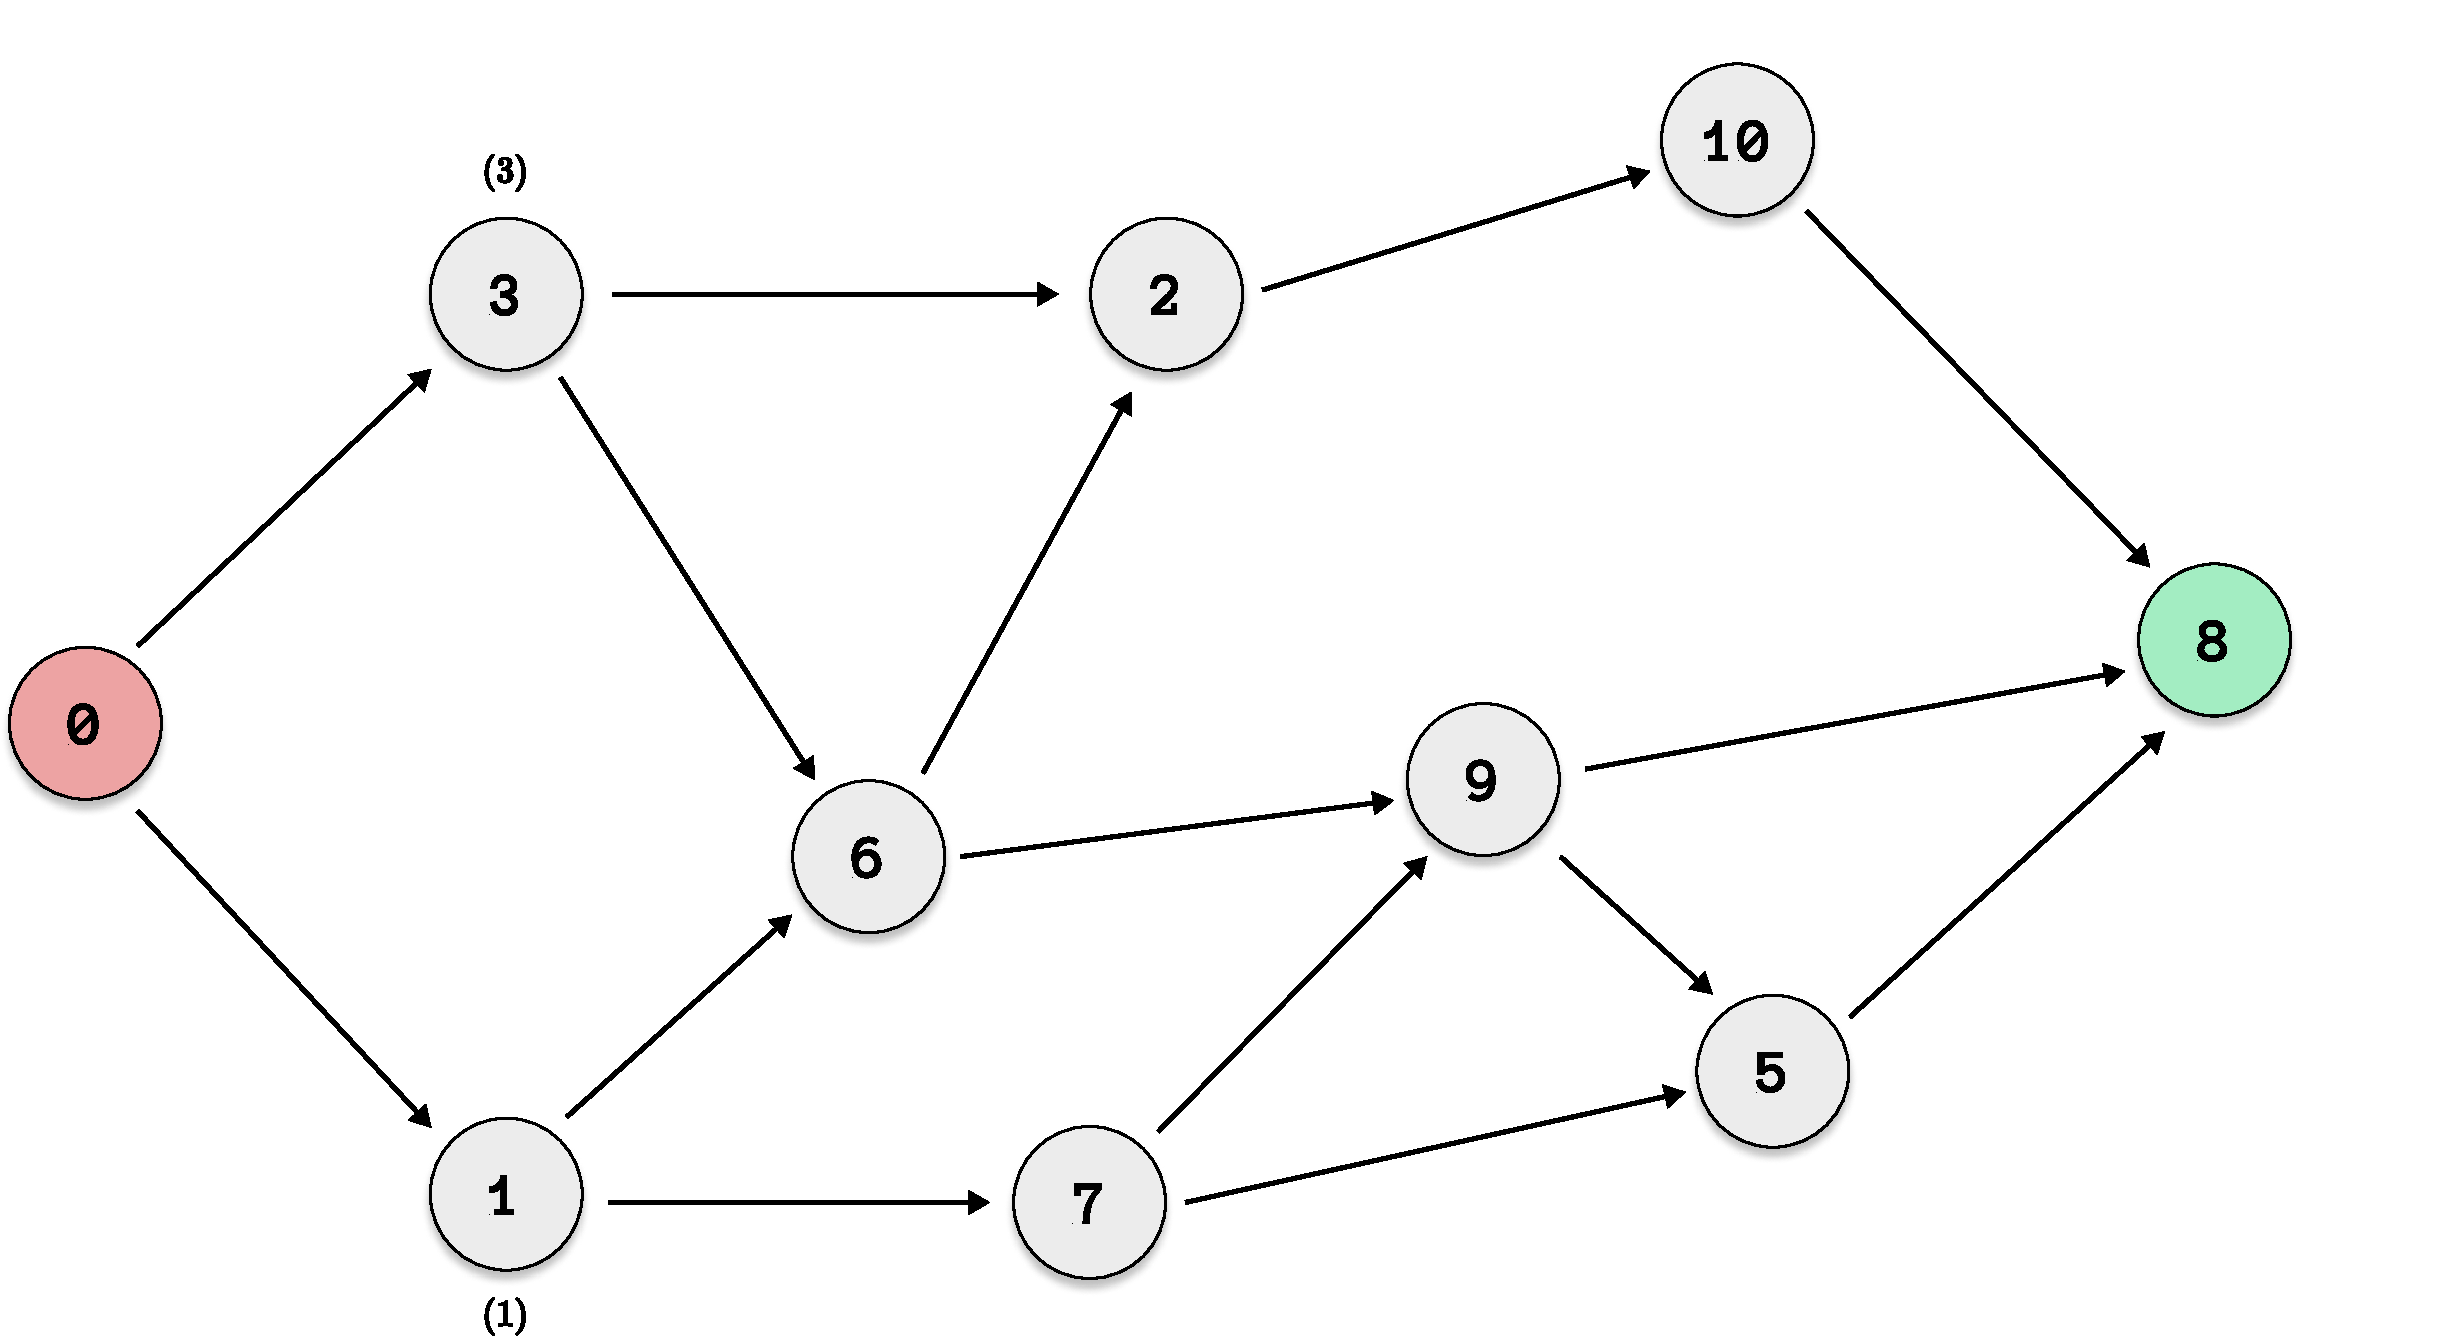
\includegraphics[width=0.85\textwidth]{assets/dag_explicit2.pdf}}
        \only<2>{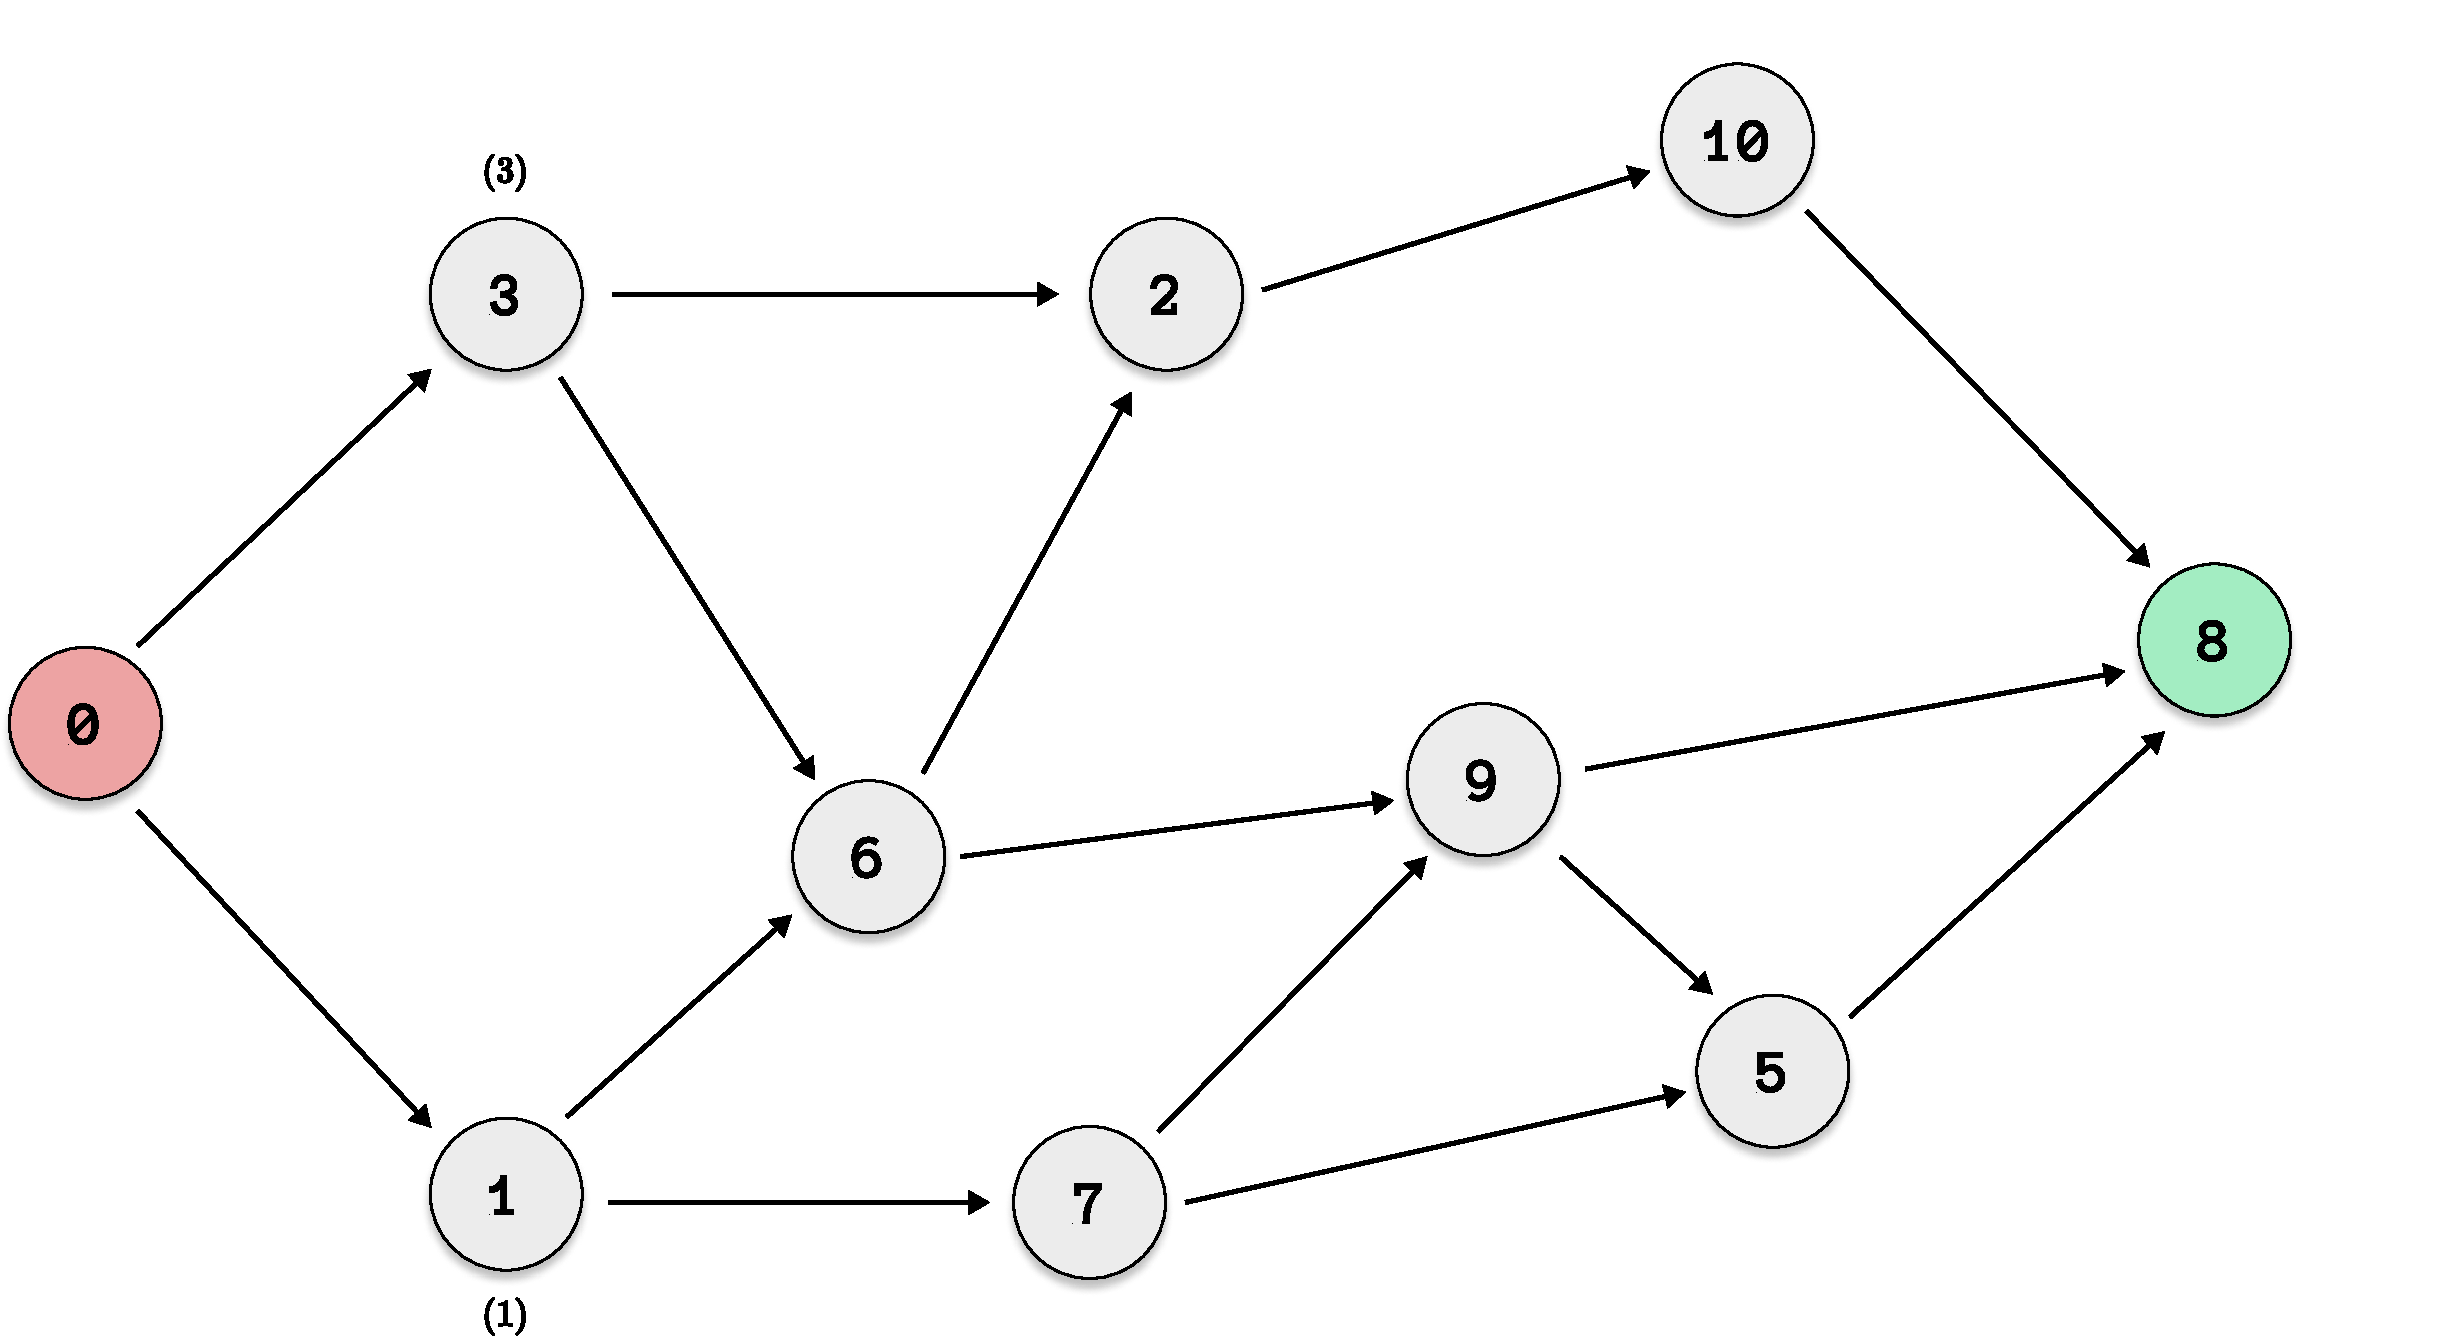
\includegraphics[width=0.85\textwidth]{assets/dag_explicit3.pdf}}
        \only<3>{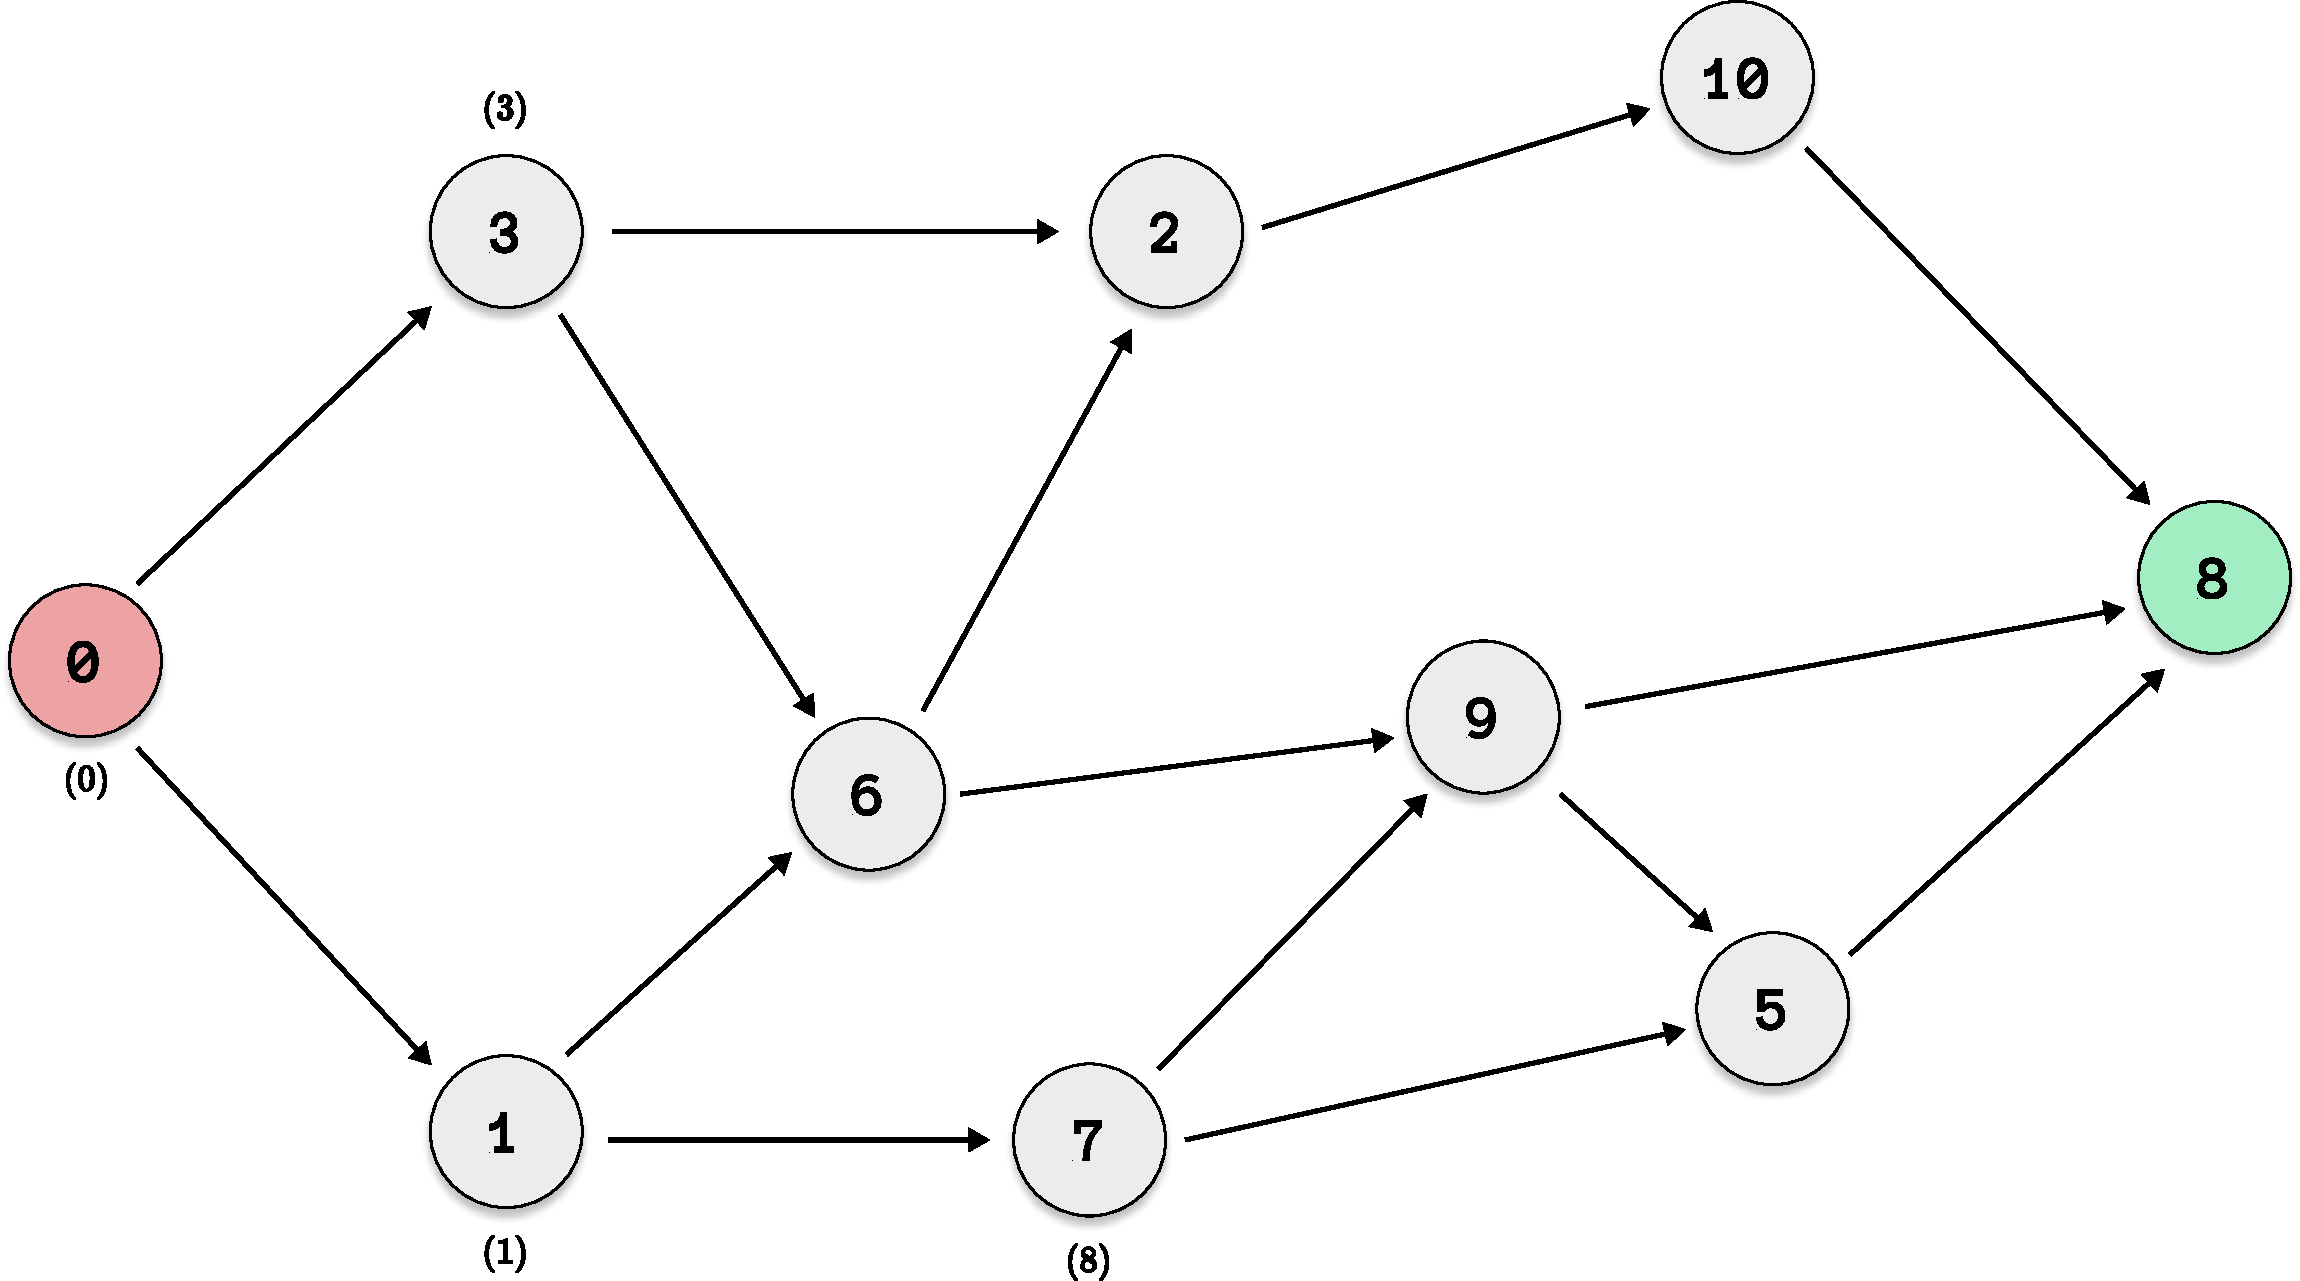
\includegraphics[width=0.85\textwidth]{assets/dag_explicit4.pdf}}
        \only<4>{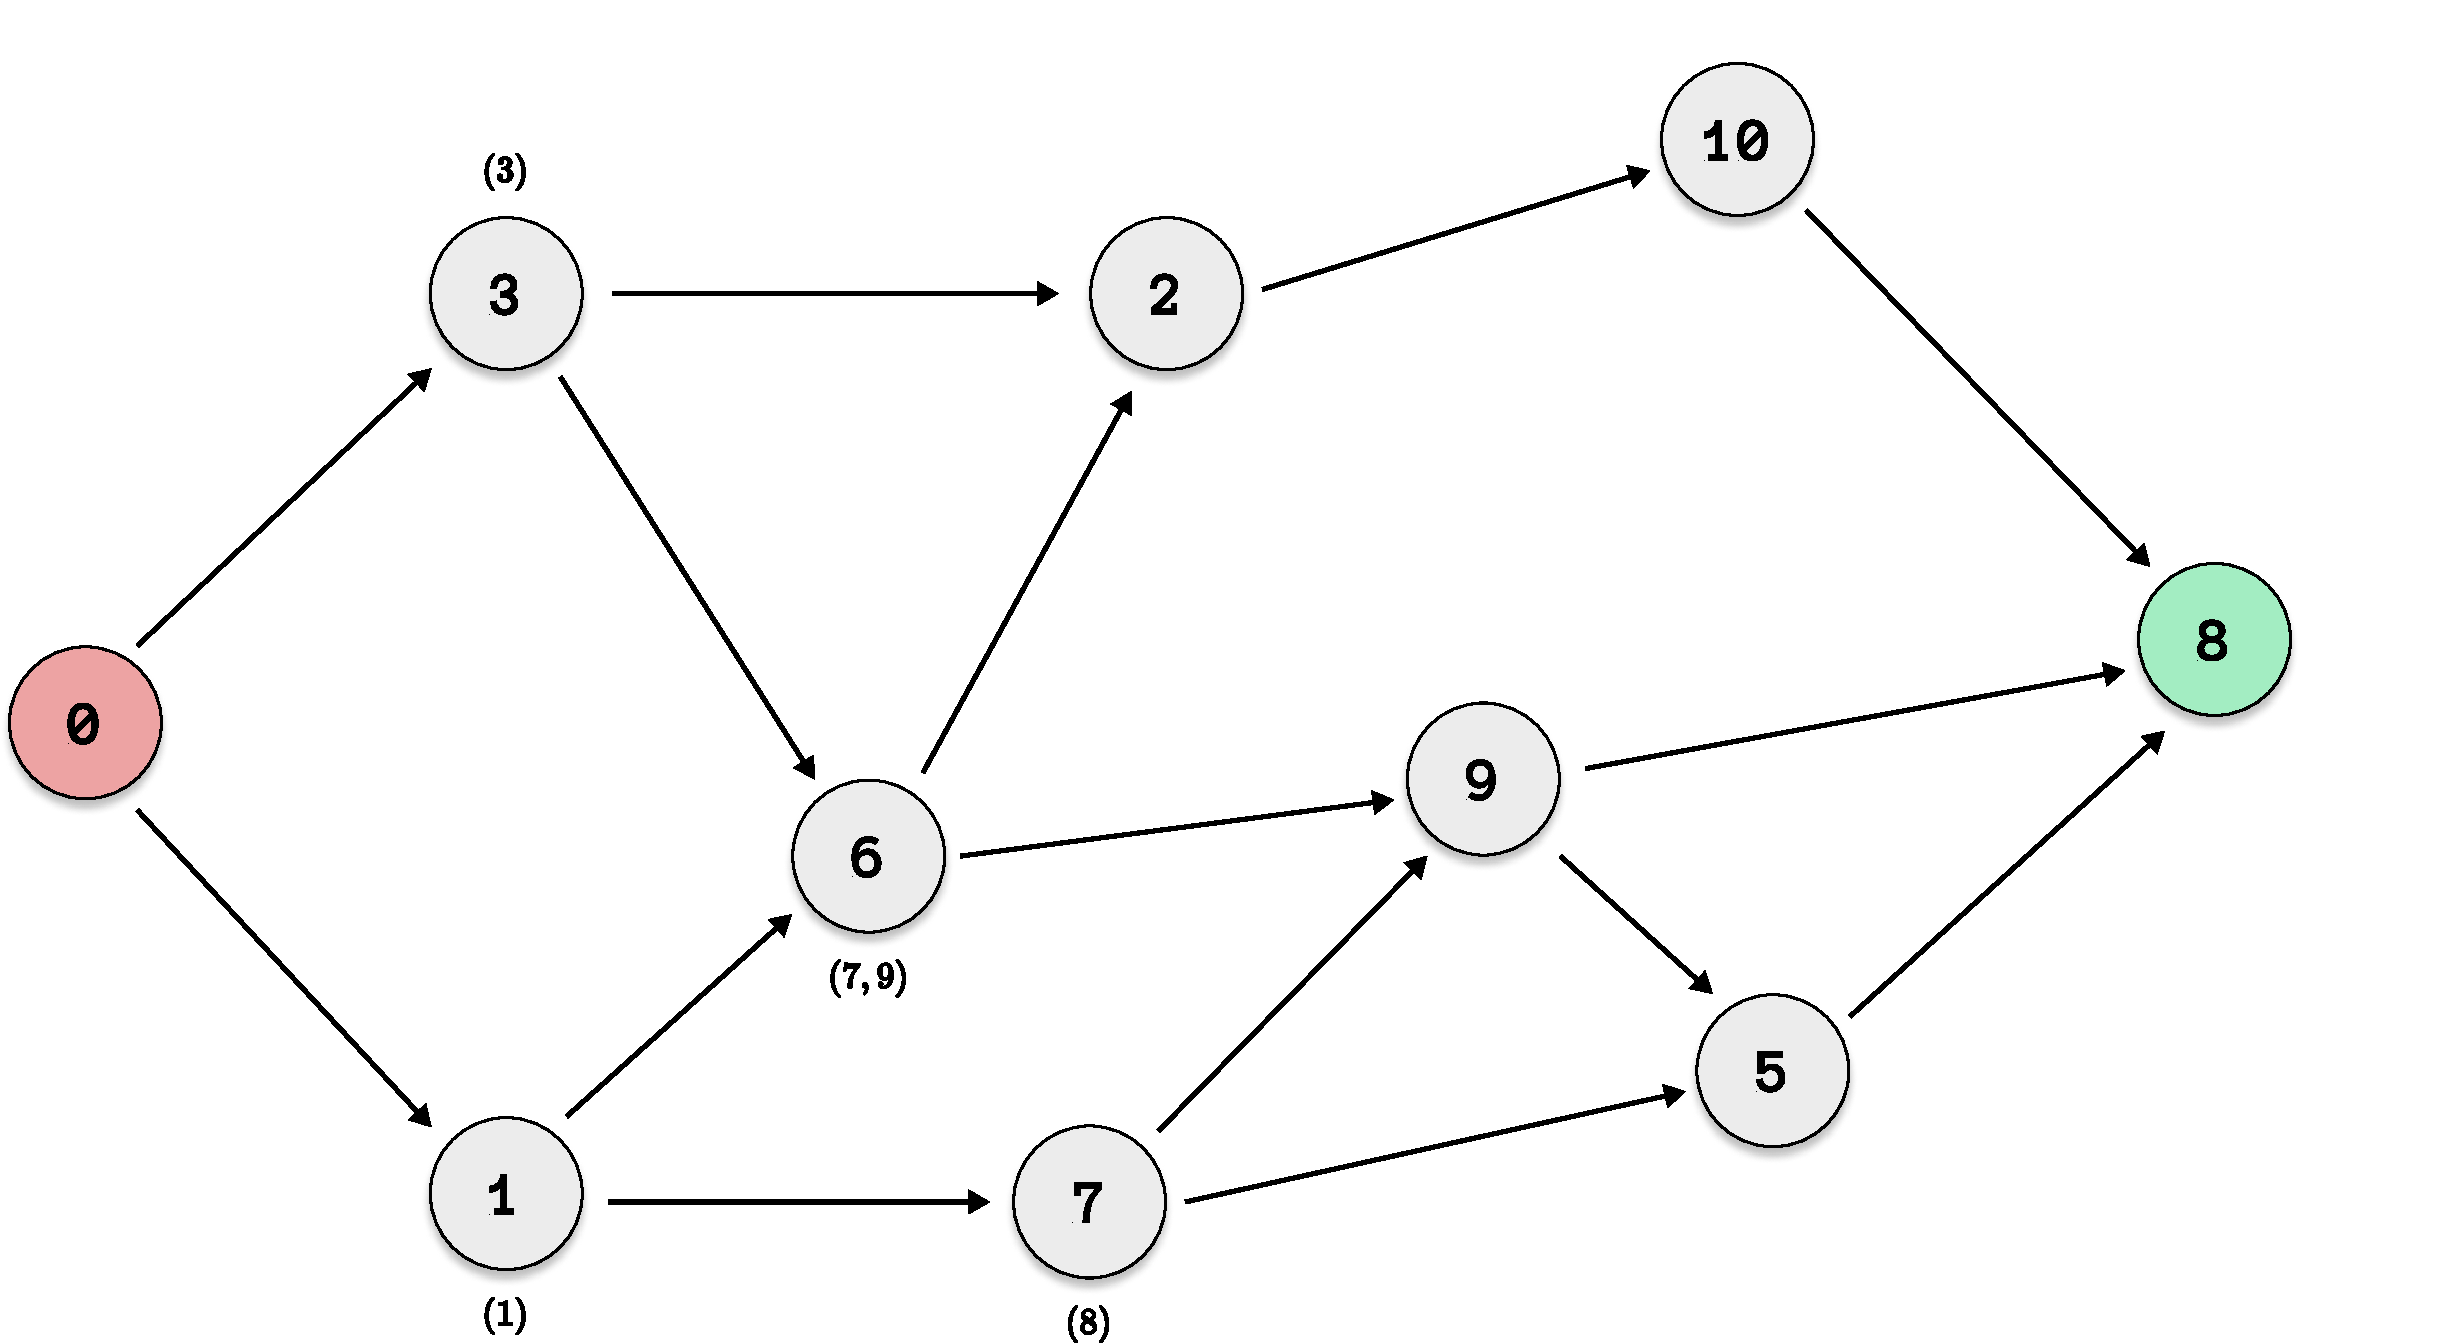
\includegraphics[width=0.85\textwidth]{assets/dag_explicit5.pdf}}
        \only<5>{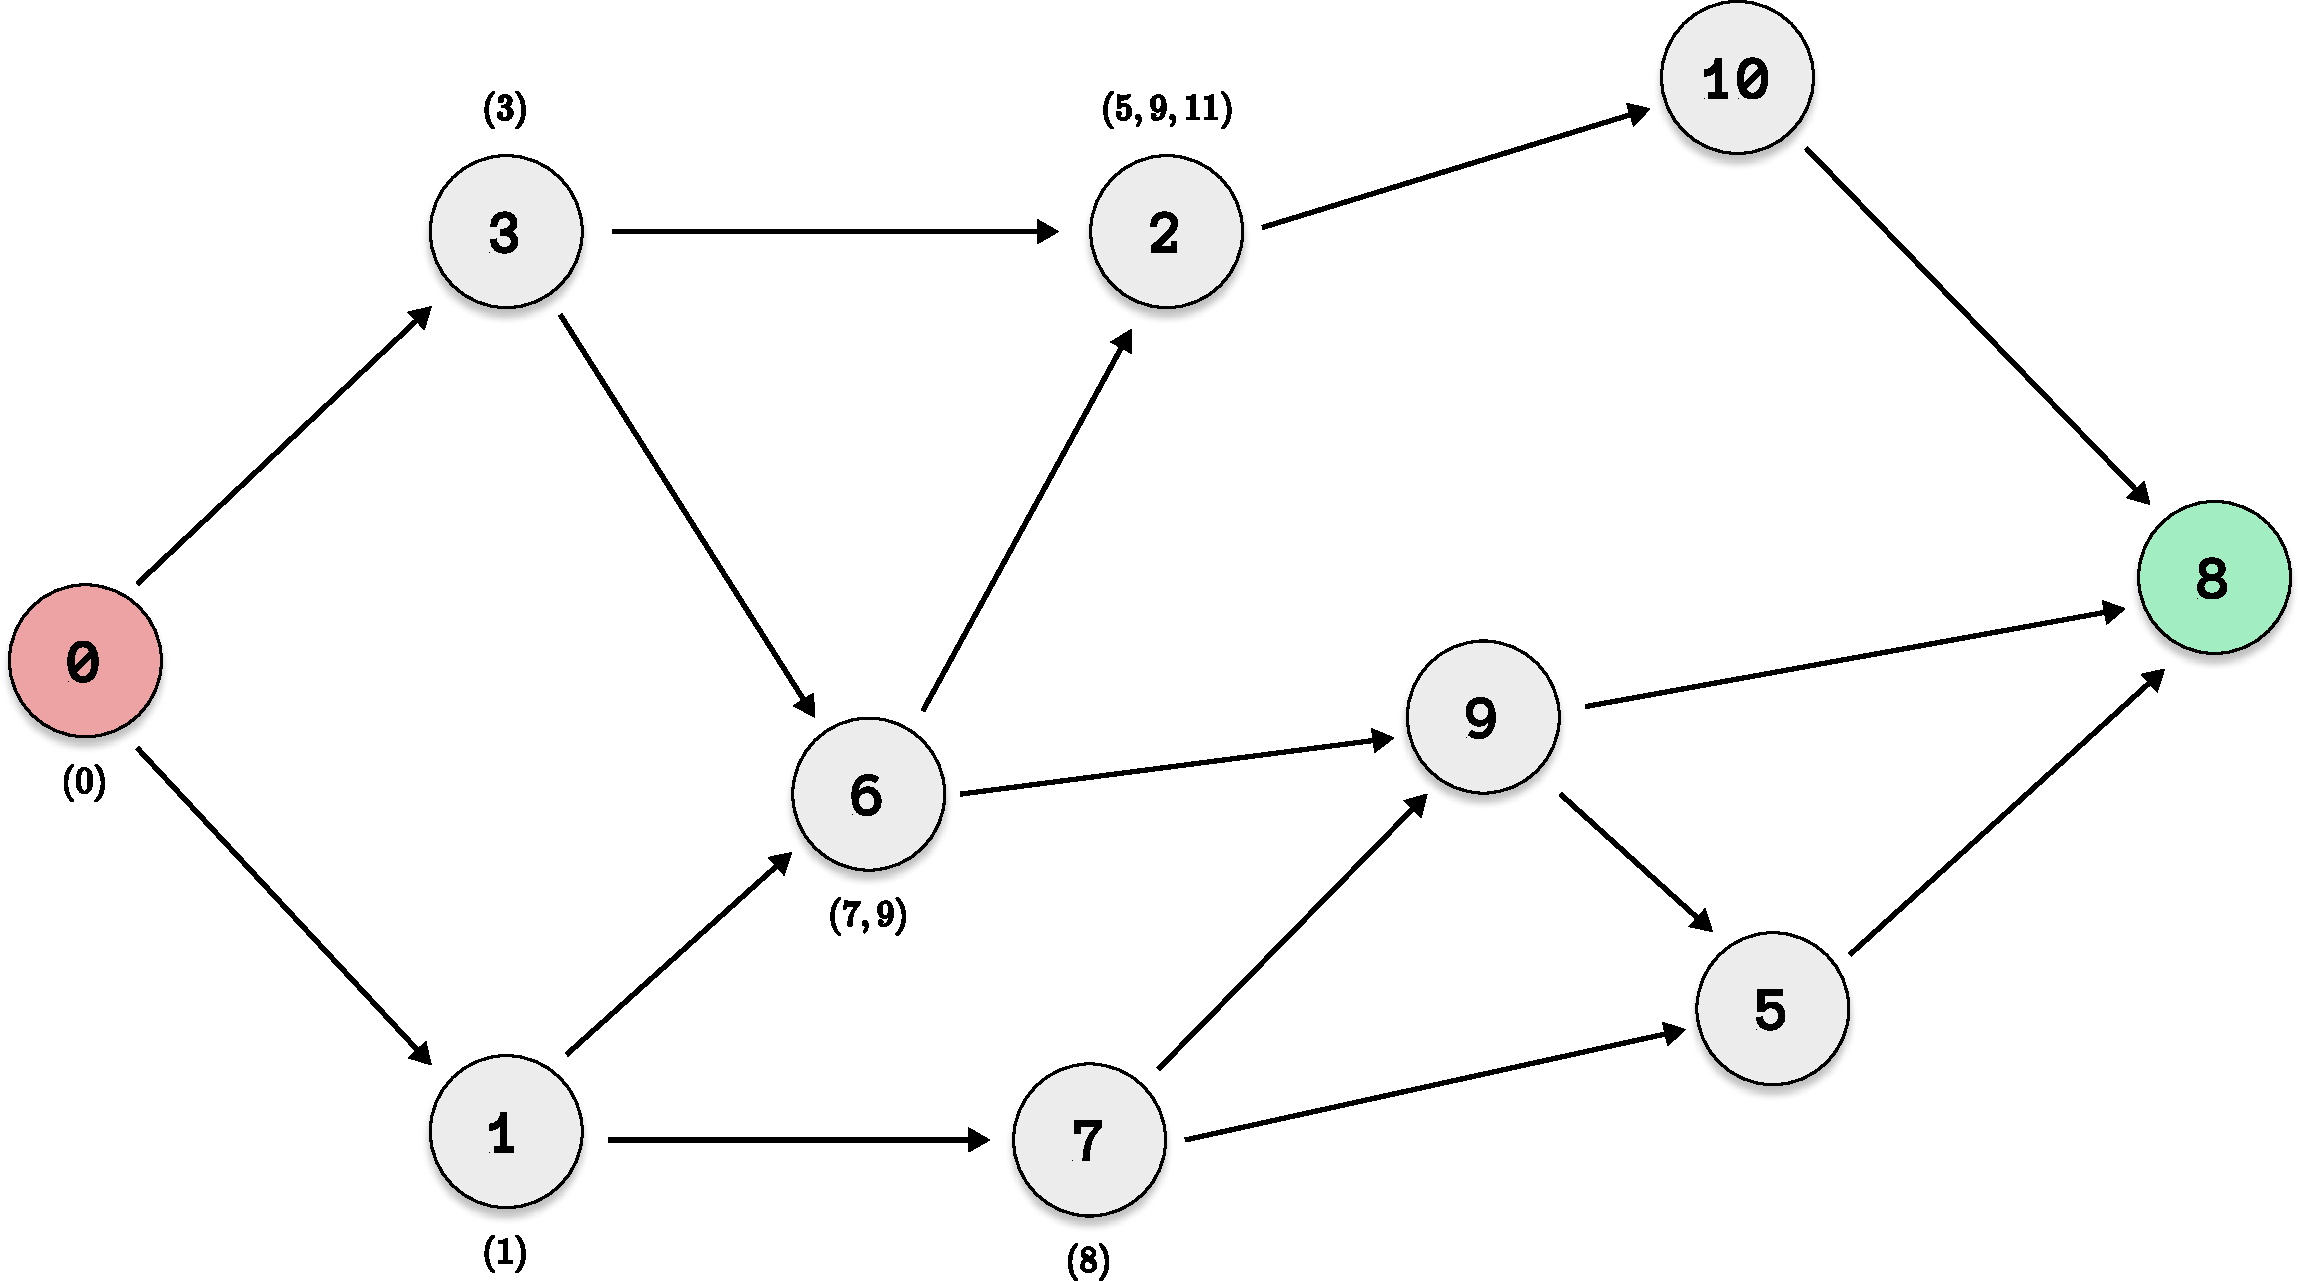
\includegraphics[width=0.85\textwidth]{assets/dag_explicit6.pdf}}
        \only<6>{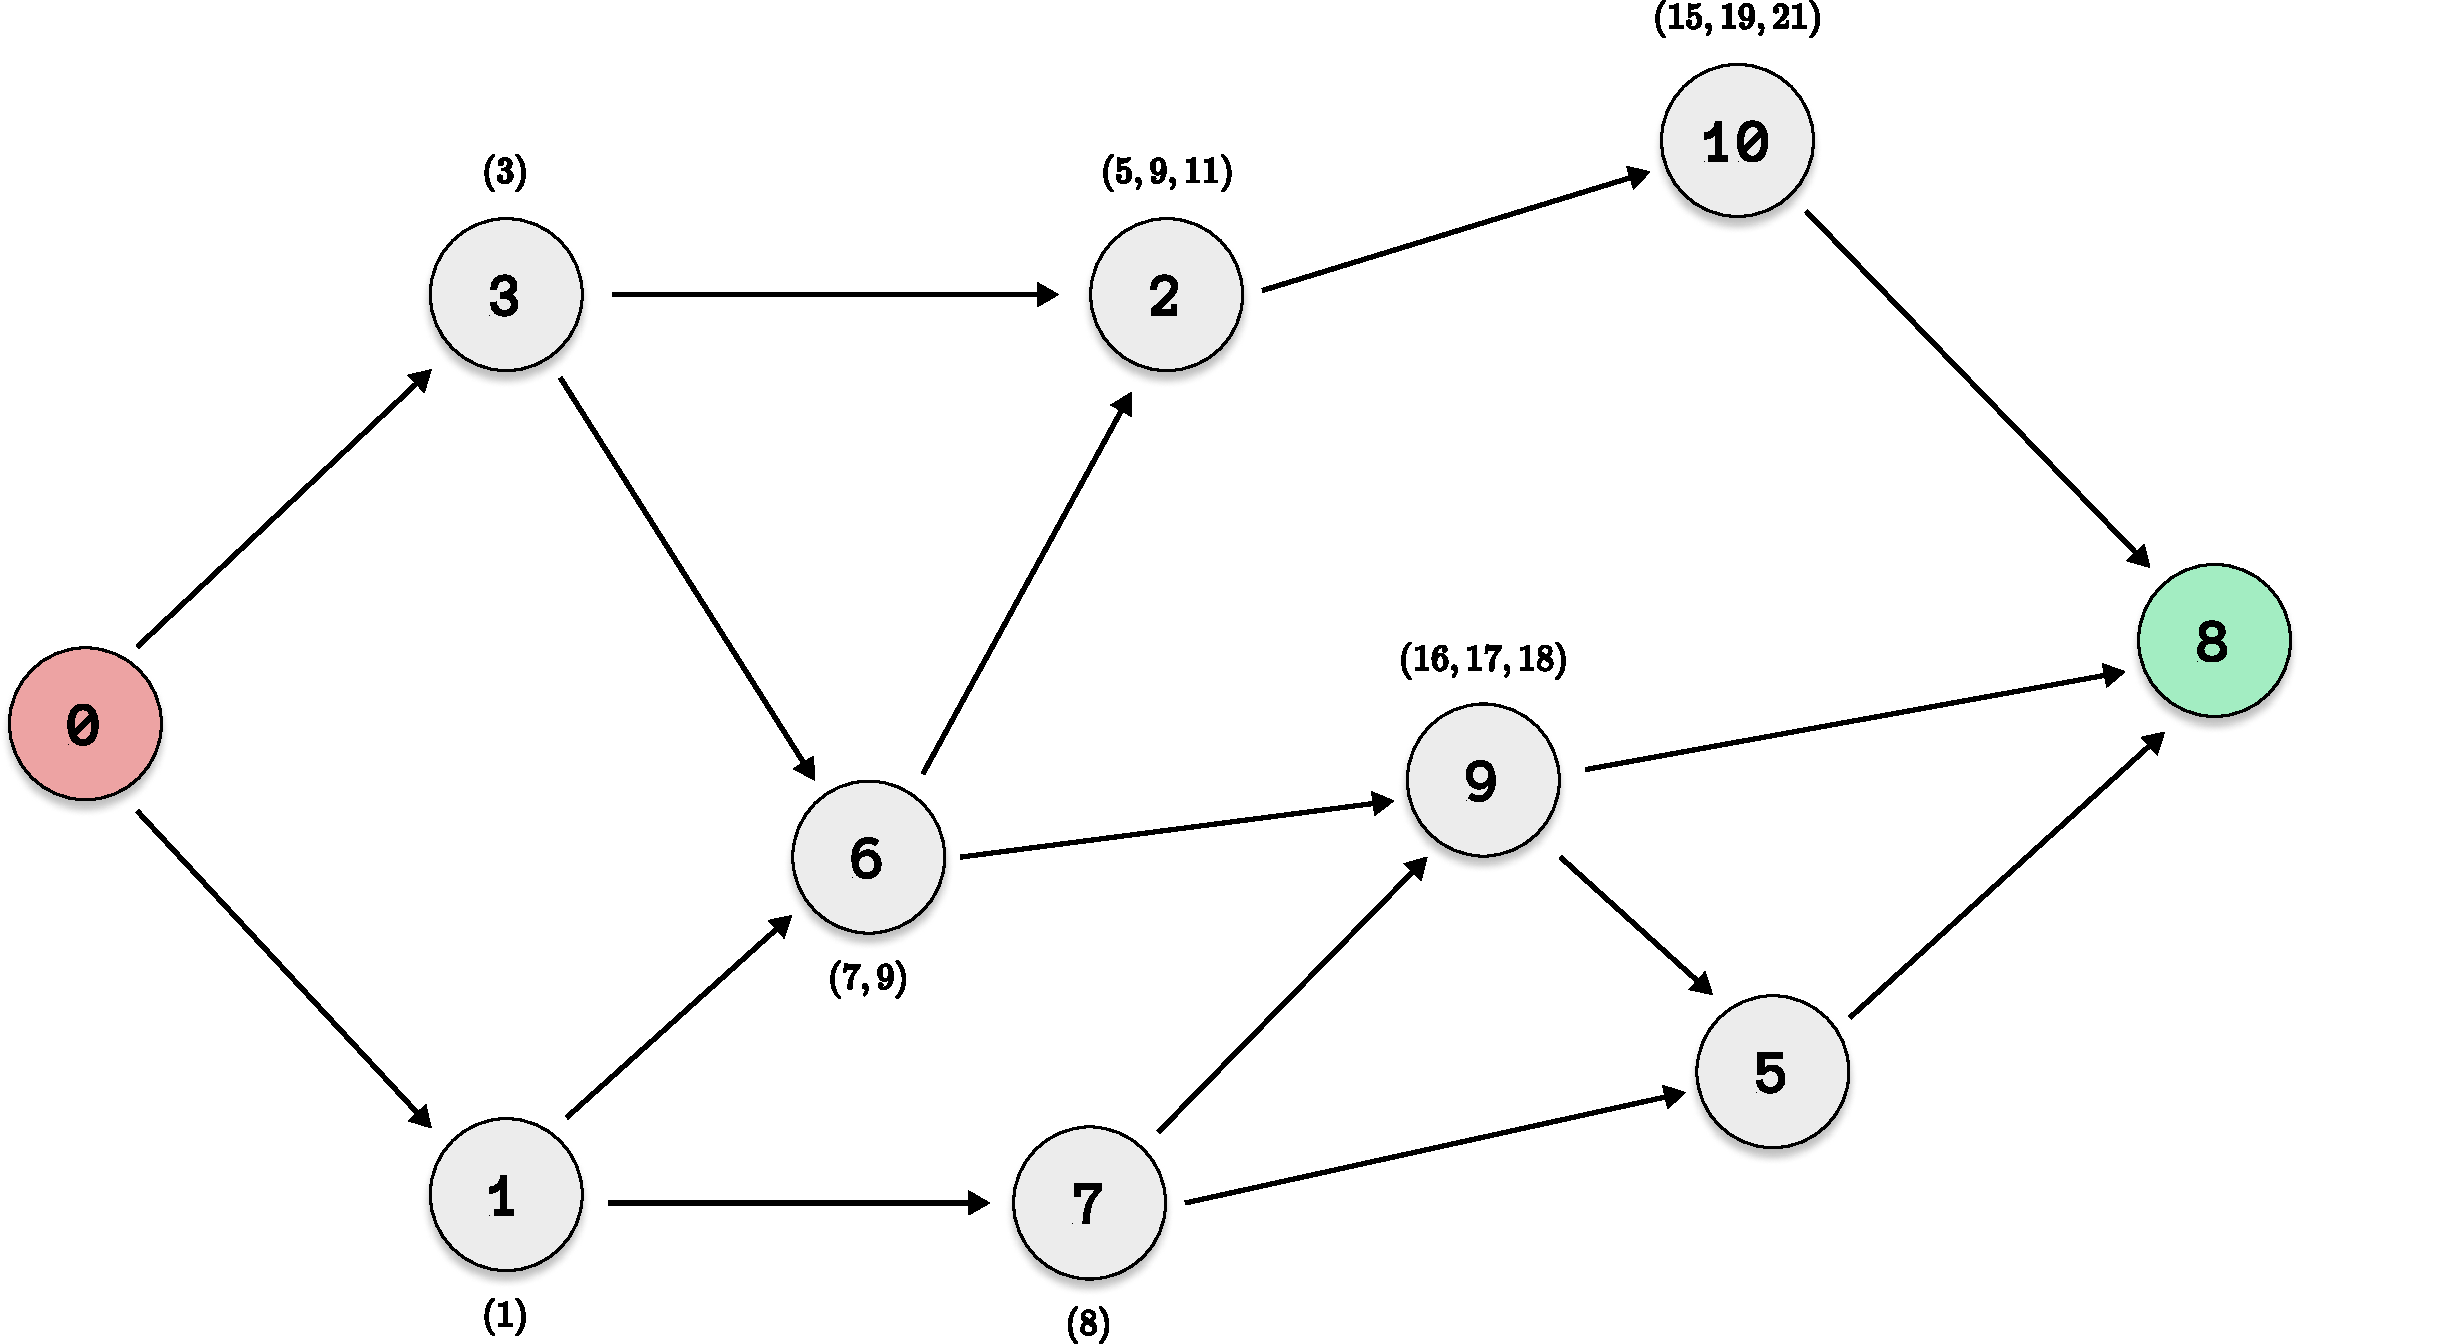
\includegraphics[width=0.85\textwidth]{assets/dag_explicit7.pdf}}
        \only<7>{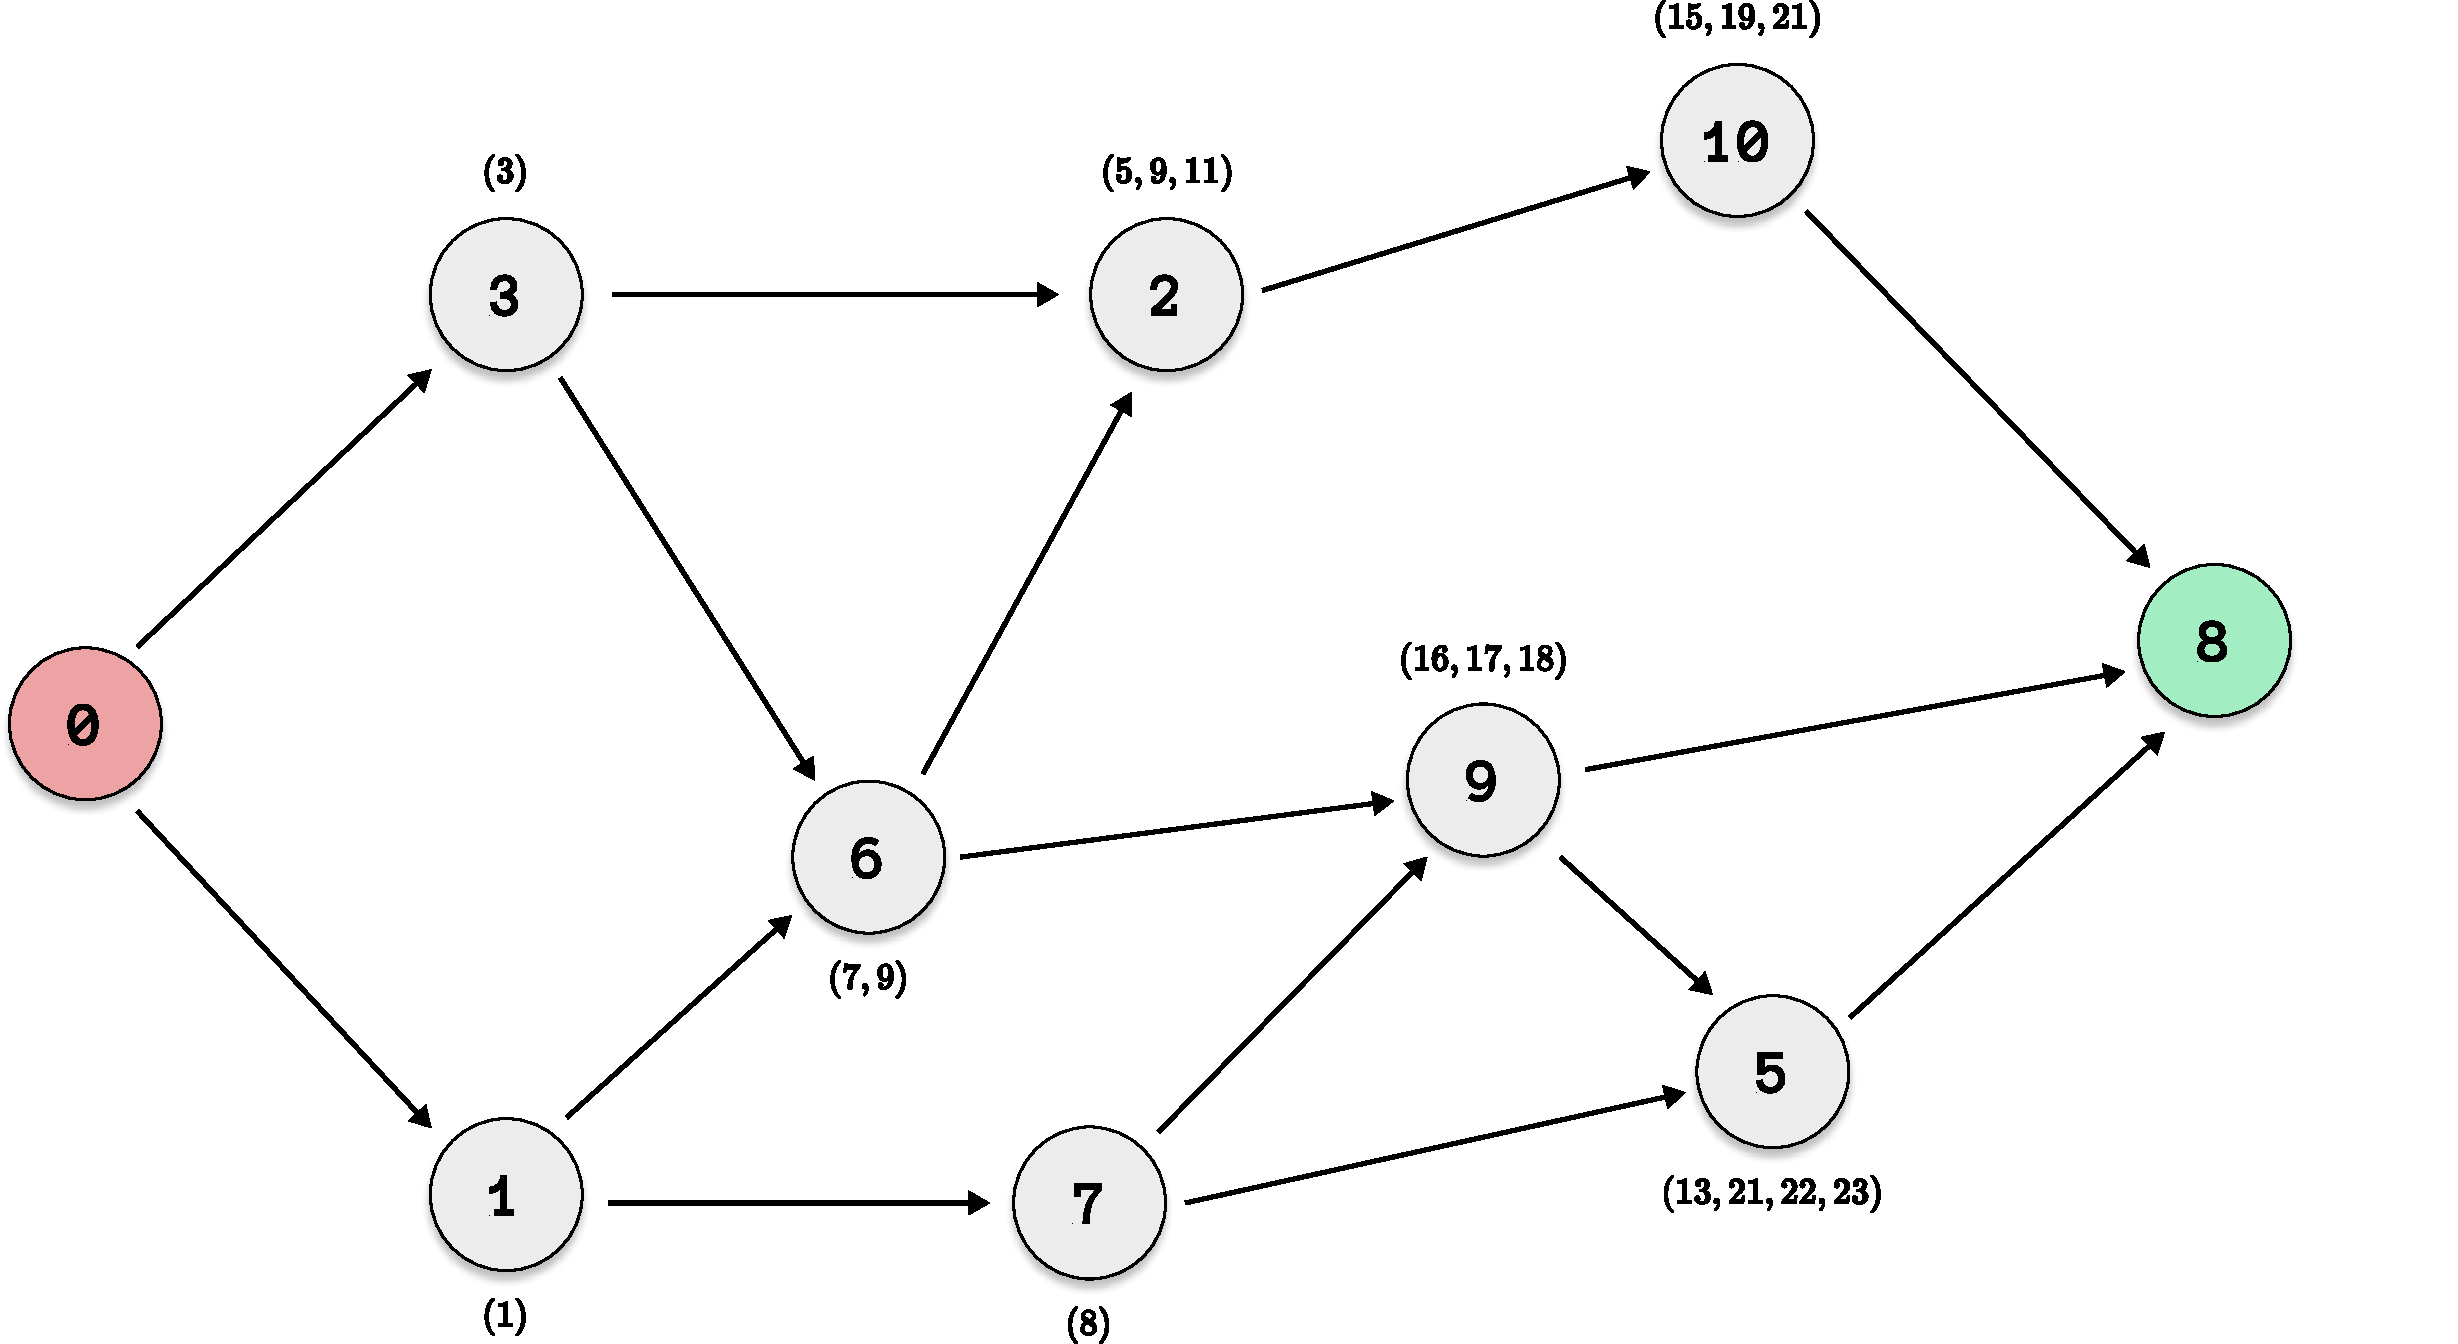
\includegraphics[width=0.85\textwidth]{assets/dag_explicit8.pdf}}
        \only<8>{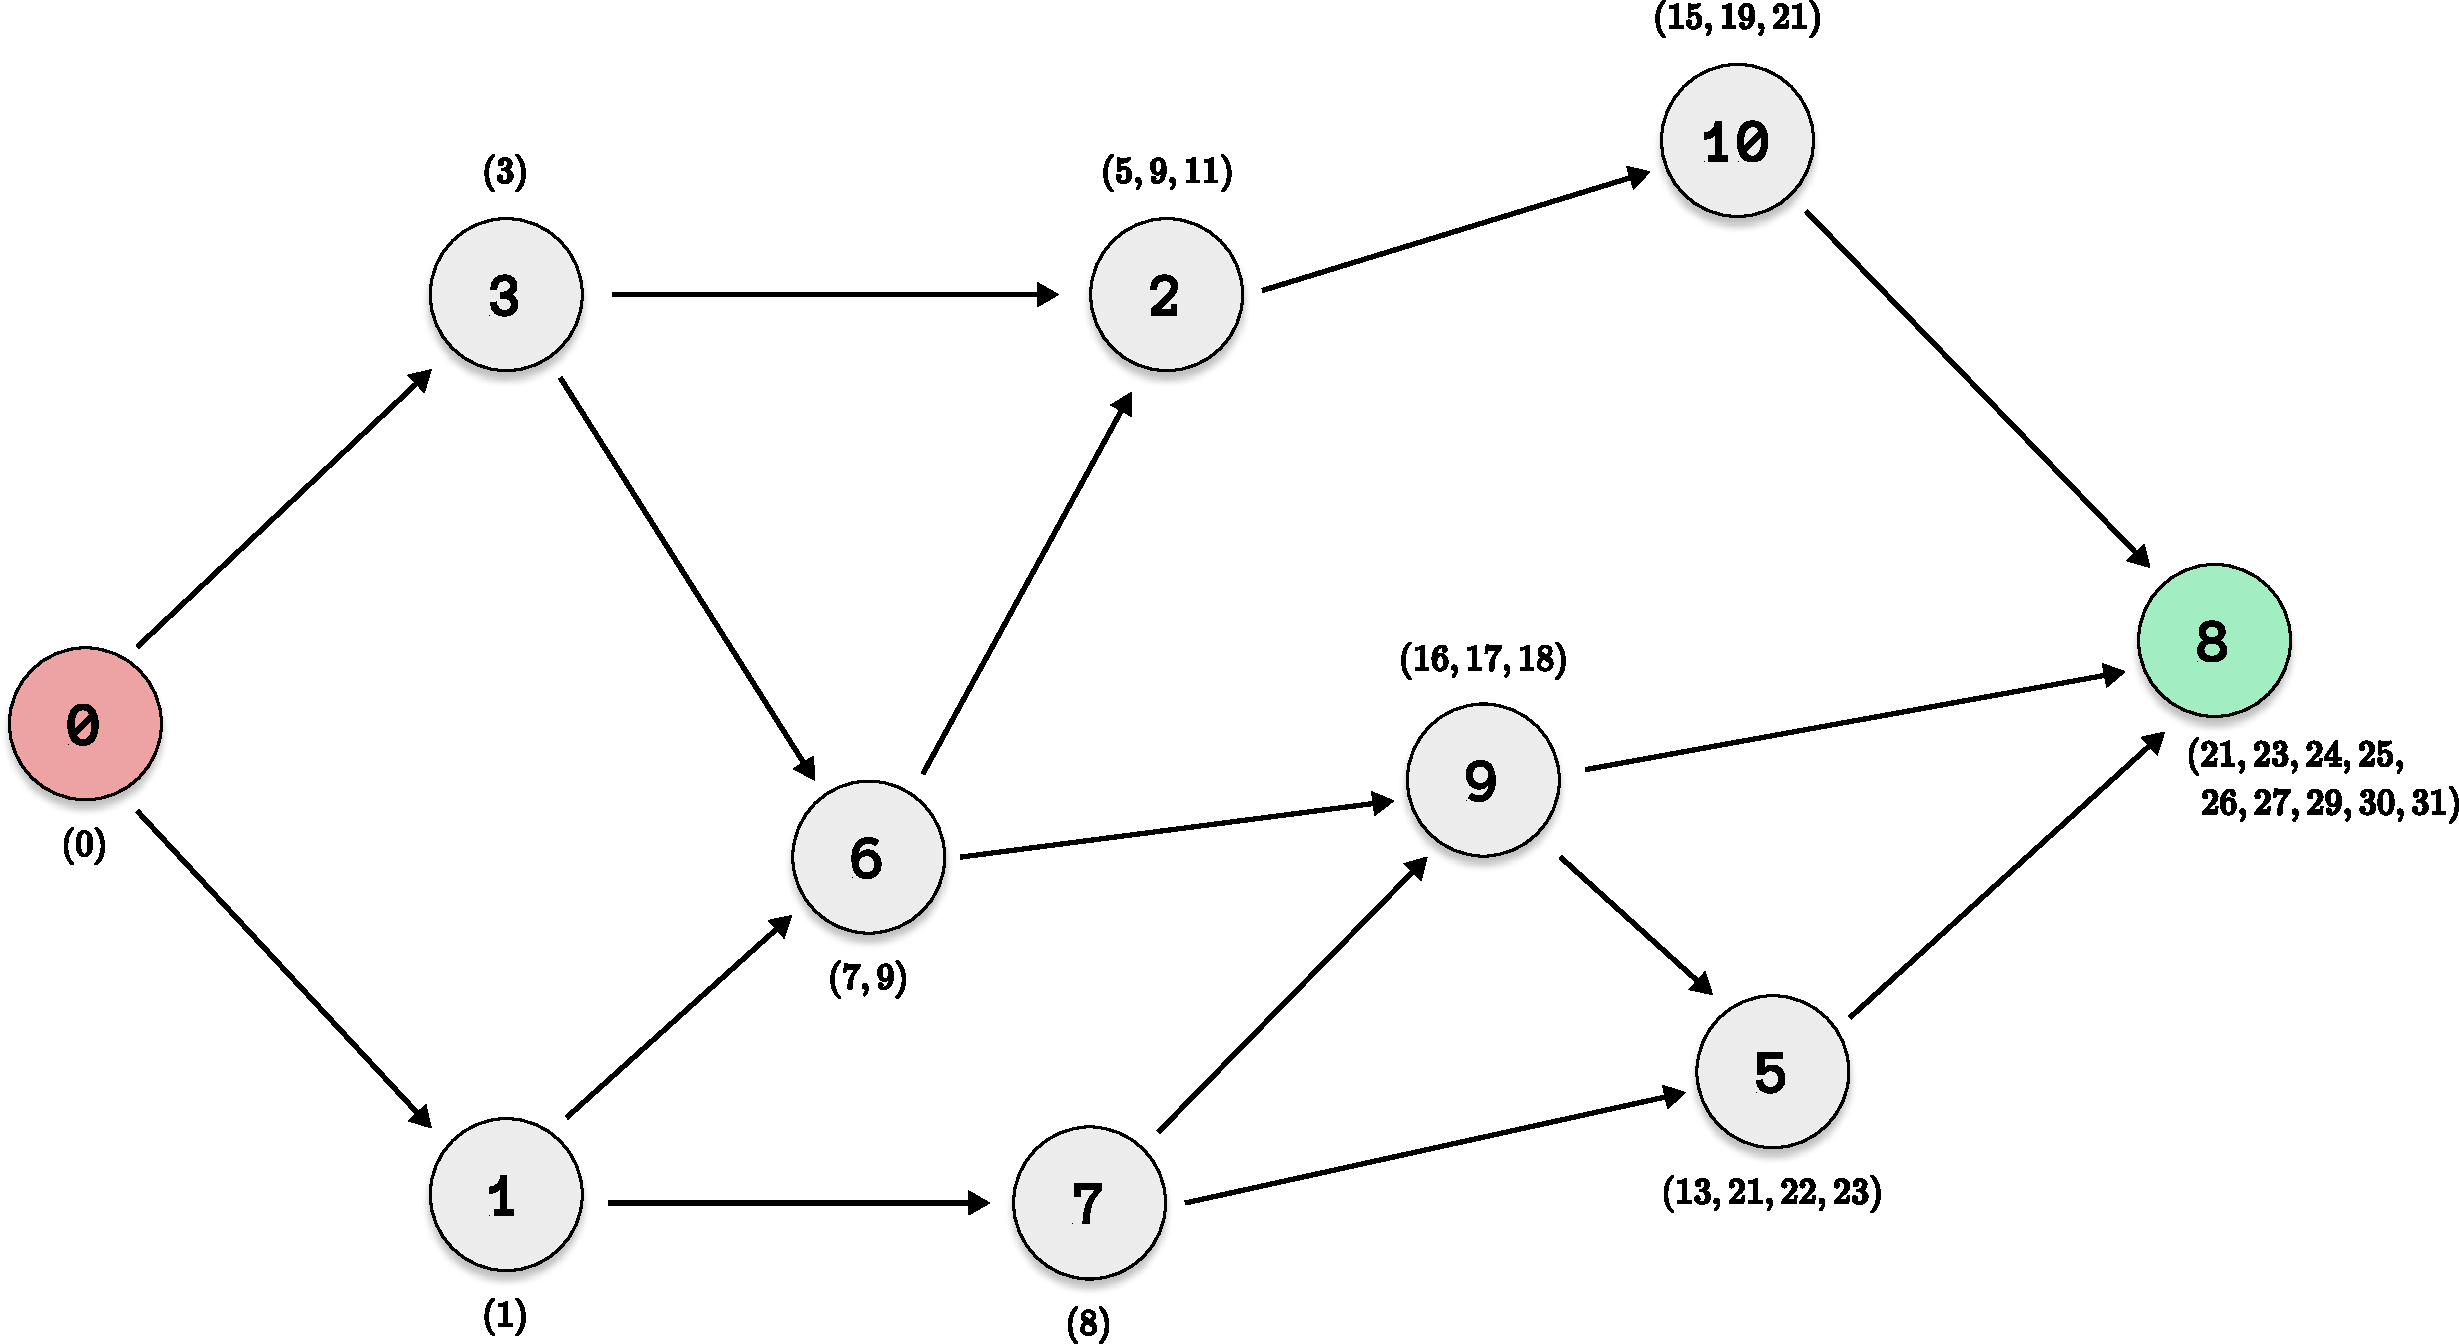
\includegraphics[width=0.85\textwidth]{assets/dag_explicit_final.pdf}}
    \end{figure}
    % \begin{figure}[h!]
    %     \centering
    %     % \resizebox{0.9\textwidth}{!}{% Reduced size slightly to make space for labels
    %     %     \begin{tikzpicture}[
    %     %         node distance=1.5cm and 1cm,
    %     %         base_node/.style={circle, draw=black, thick, minimum size=8mm, inner sep=0pt, font=\sffamily},
    %     %         root_node/.style={base_node, fill=red!60, text=black},
    %     %         % Definizione stile per label O-set
    %     %         data_label/.style={font=\tiny\ttfamily, text=blue!80!black, anchor=north},
    %     %         edge_style/.style={->, >={Stealth[length=2mm]}, thick, draw=black}
    %     %         ]

    %     %         % Nodes (pesi dentro)
    %     %         \node[root_node] (0) at (0, 2) {0};
    %     %         \node[base_node] (1) at (1.5, 0) {1};
    %     %         \node[base_node] (3) at (1.5, 4) {3};
    %     %         \node[base_node] (6) at (3.5, 1.5) {6};
    %     %         \node[base_node] (7) at (4.5, 0) {7};
    %     %         \node[base_node] (2) at (5.5, 4) {2};
    %     %         \node[base_node] (9) at (6.5, 2) {9};
    %     %         \node[base_node] (5) at (9, 0.5) {5};
    %     %         \node[base_node] (10) at (8.5, 5) {10};
    %     %         \node[base_node] (8) at (11, 3) {8};

    %     %         % Edges
    %     %         \draw [edge_style] (0) -- (1); \draw [edge_style] (0) -- (3);
    %     %         \draw [edge_style] (1) -- (6); \draw [edge_style] (1) -- (7);
    %     %         \draw [edge_style] (3) -- (2); \draw [edge_style] (3) -- (6);
    %     %         \draw [edge_style] (6) -- (2); \draw [edge_style] (6) -- (9);
    %     %         \draw [edge_style] (7) -- (5); \draw [edge_style] (7) -- (9);
    %     %         \draw [edge_style] (2) -- (10);
    %     %         \draw [edge_style] (9) -- (5); \draw [edge_style] (9) -- (8);
    %     %         \draw [edge_style] (10) -- (8); \draw [edge_style] (5) -- (8);

    %     %         % O-Set Labels appearing step-by-step
    %     %         \node<1->[data_label, red] at (0.south) {\{0\}};
    %     %         \node<2->[data_label] at (1.south) {\{1\}};
    %     %         \node<2->[data_label] at (3.south) {\{3\}};
    %     %         \node<3->[data_label] at (7.south) {\{8\}};
    %     %         \node<4->[data_label] at (6.south) {\{7, 9\}};
    %     %         \node<5->[data_label] at ([xshift=0.3cm]2.south) {\{5, 9, 11\}};
    %     %         \node<6->[data_label] at ([yshift=-0.1cm, xshift=0.2cm]9.south) {\{16, 17, 18\}};
    %     %         \node<7->[data_label] at (10.south) {\{15, 19, 21\}};
    %     %         \node<8->[data_label] at (5.south) {\{13, 21, 22, 23\}};
    %     %         \node<9->[data_label, align=center] at ([yshift=-0.2cm, xshift=0.4cm]8.south) {\{21, 23, 24, 25, \\ 26, 27, 29, 30, 31\}};

    %     %     \end{tikzpicture}
    %     % } % End resizebox
    % \end{figure}
\end{frame}

% --- SLIDE 15: The Rank Query - Concept ---
\begin{frame}{The Rank Query on Weighted DAGs}
    \framesubtitle{What Values are "Active" at Node N?}
    % \begin{block}{Motivation}
    %     The $\mathcal{O}$-Set ($\mathcal{O}_N$) tells us the \alert{final} path weights ending at node $N$.
    %     But we want to know which cumulative weight values are relevant \alert{during} the "processing" step associated with node $N$ itself.
    % \end{block}
    \begin{block}{Rank Query on a Node $N$: $\mathrm{rank}_G(N)$}
        \begin{enumerate}
            \item Returns a representation of a set of integers derived from the $\mathcal{O}$-set $\mathcal{O}_N$.
                  \[ S_N = \bigcup_{x \in \mathcal{O}_N} \{ z \in \mathbb{N}_0 \mid \max(0, x - w(N) + 1) \le z \le x \}. \]
                  \vspace{-1em}
                  \pause
            \item These intervals are then maximally merged. The query $\mathrm{rank}_G(N)$ returns a \alert{minimal collection of disjoint closed integer intervals}
                  \[ \mathcal{R}_N = \{[l_1, r_1], [l_2, r_2], \dots, [l_p, r_p]\} \]
                  such that their union exactly covers $S_N$.
                  % \item Return the result as a \alert{minimal set of disjoint intervals} $\mathcal{R}_N$.
        \end{enumerate}
    \end{block}
    $\mathcal{R}_N$ captures the range of possible cumulative sums during the \emph{activity} at node $N$

\end{frame}
